\section{Introduction}
\label{sec:intro}

Computational pathology now includes models trained directly from gigapixel whole-slide images (WSIs), often using only a slide-level diagnosis. Such models have been applied to cancer detection and subtyping, weakly supervised slide classification, and prediction of molecular biomarkers from H\&E tissue~\cite{campanella2019clinical,lu2021clam,kather2019msi,shmatko2022ai}. Large pretrained encoders have widened the set of tasks that can be studied with limited labels. CTransPath uses contrastive pretraining; UNI and Virchow learn visual representations from large slide collections; CONCH pairs pathology images with text; and Prov-GigaPath incorporates long-range WSI context~\cite{wang2022ctranspath,chen2024uni,lu2024conch,vorontsov2024virchow,xu2024gigapath}. The evidence used by these models is still difficult to inspect.

H\&E images mix tissue biology with choices made during fixation, staining, scanning, and compression. Nuclear shape, cell density, and tumor--immune organization can all correlate with stain intensity or source institution. Howard \etal{} found that site-specific signatures remain detectable after commonly used normalization and augmentation procedures~\cite{howard2021sitespecific}. A model can therefore perform well on a held-out set while relying partly on acquisition cues. This is one reason post-hoc explanations in medical AI require careful validation~\cite{ghassemi2021falsehope,klauschen2024xai}.

Saliency and attention maps provide spatial localization, but the contents of a highlighted region are rarely unambiguous. A tumor region may be influential because of nuclear size, immune density, spatial mixing, stain, or a scanner artifact. Adebayo \etal{} also showed that some saliency maps remain visually similar after randomizing model parameters or training labels~\cite{adebayo2018sanity}. In a pathology image, knowing where a response occurs does not identify the tissue property responsible for it.

Visual counterfactuals give a more direct test by modifying the input and measuring the resulting prediction. Goyal \etal{} retrieve discriminative changes relative to a target class~\cite{goyal2019counterfactual}. DVCE, DiME, and DiG-IN use diffusion priors to produce realistic classifier-guided edits~\cite{augustin2022dvce,jeanneret2022dime,augustin2024digin}. Pathology-specific studies have generated class transitions that expose morphology associated with molecular labels~\cite{dolezal2023synthetic}. MoPaDi is the closest example to our setting: a diffusion autoencoder is coupled to a task-specific classifier or multiple-instance model to produce morphological counterfactuals~\cite{zigutyte2026mopadi}. Its edits are optimized toward a target prediction. Several correlated attributes may change in the process, which makes it hard to assign the model response to one requested factor.

\begin{figure}[!t]
    \centering
    \vspace{2mm}
    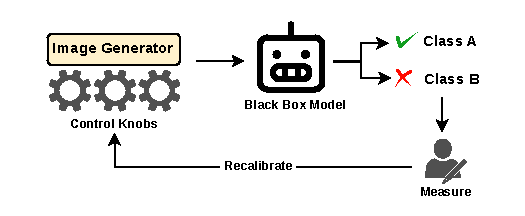
\includegraphics[width=\columnwidth]{../Figure1.pdf}
    \vspace{-6mm}
    \caption{Counterfactual probing with matched, single-control interventions.}
    \label{fig:probing_cartoon}
\end{figure}

\method{} starts from a requested intervention rather than a target prediction (Fig.~\ref{fig:probing_cartoon}). A latent diffusion model receives a dense cellular map and a 16-dimensional morphology/appearance vector. The five map channels specify the position and density of tumor, inflammatory, epithelial, connective/stromal, and necrotic compartments through dense spatial conditioning~\cite{zhang2023controlnet}. Blockwise feature-wise linear modulation (FiLM) controls summaries of nuclear geometry, texture, and RGB appearance~\cite{perez2018film}. Images in a counterfactual pair use the same initial noise and retain every non-intervened condition. Each requested change is measured in the generated image before the pair is used to probe a model.

The evaluation reflects that use case. FID and KID measure distributional realism, while recovered cell counts, centroid matches, and morphology measurements test whether the generator followed its conditions. Candidate selection uses \cellvit{}; independent measurements from \hovernet{} and \stardist{} expose any gain that depends on the in-loop analyzer~\cite{horst2026cellvitpp,graham2019hovernet,schmidt2018stardist}. Training uses 1.4 million WSI tiles of size $n\!\times\!n$, with $n=512$, sampled from 1,096 whole-slide images (one patient per WSI). Accepted pairs can then be reused across pathology encoders, task-specific classifiers, and survival models without changing the generation procedure.

The paper makes four technical contributions:
\begin{itemize}
    \item a conditional latent-diffusion architecture for $512\!\times\!512$ H\&E synthesis, with dense cellular maps and blockwise FiLM controls;
    \item a same-noise protocol for interventions on spatial organization, morphology, or appearance while the other modeled conditions remain fixed;
    \item a fixed-budget seed-selection procedure based on agreement between the requested and recovered cellular maps, with realism reported before and after selection; and
    \item a fidelity audit using three cell-analysis models, followed by counterfactual tests that are independent of the prediction being studied.
\end{itemize}
